\subsection{Задание 1}%
\label{subsec:1}%
Исходные данные неупорядоченные:\newline%
\newline%
%
\begin{changemargin}{-4cm}{0cm}\small{%
\begin{tabular}{|p{0.08\linewidth}|p{0.08\linewidth}|p{0.08\linewidth}|p{0.08\linewidth}|p{0.08\linewidth}|p{0.08\linewidth}|p{0.08\linewidth}|p{0.08\linewidth}|p{0.08\linewidth}|p{0.08\linewidth}|}%
\hline%
0.24120&0.20069&2.49827&0.34931&0.70002&1.02003&0.13744&0.41287&0.18402&1.50855\\%
\hline%
0.50039&0.32609&0.25789&0.08005&0.02970&0.69878&0.03860&0.13562&0.94595&0.79714\\%
\hline%
1.07189&2.04207&0.55176&0.13330&0.04860&0.09261&0.73266&0.39373&0.03471&0.59748\\%
\hline%
0.00550&0.10785&0.48580&0.12093&1.23308&0.40318&0.59348&0.15540&0.01085&0.65834\\%
\hline%
0.46964&0.57113&0.33739&0.78320&0.61860&0.09328&0.05437&0.27422&0.13480&0.55982\\%
\hline%
0.16836&0.08466&0.03538&0.68691&0.31945&0.32272&0.95414&0.00067&0.78717&0.59659\\%
\hline%
0.55605&2.15305&0.49415&0.02424&0.89349&0.80630&0.37284&0.31772&0.04112&0.32601\\%
\hline%
0.26923&0.12576&0.07903&0.03152&0.41632&0.04060&0.13879&0.12846&0.01667&0.72244\\%
\hline%
0.54765&0.16667&0.07035&0.02681&0.54523&0.53271&0.45727&0.19646&0.46272&0.90750\\%
\hline%
0.67340&0.10823&0.04123&0.68070&0.07748&0.11075&0.18493&0.13457&1.18247&0.38154\\%
\hline%
0.06569&0.16240&0.04554&0.80698&0.26408&0.18152&0.02194&0.01732&0.07088&0.50737\\%
\hline%
0.42889&0.34414&0.38134&0.40327&0.79952&0.27456&0.25624&0.06428&0.29408&0.36317\\%
\hline%
0.09802&0.46832&0.11789&0.03405&0.00989&0.16255&0.13362&0.35968&0.16359&0.24217\\%
\hline%
0.14683&0.00237&0.75408&0.88643&0.30986&0.31571&0.19583&0.16891&1.63331&0.12351\\%
\hline%
0.40976&0.08514&0.27008&0.37772&0.15724&0.29163&0.26879&0.09789&0.07231&0.23268\\%
\hline%
0.04717&0.38958&0.43365&1.27750&0.90610&0.75378&0.48882&0.08835&0.35536&0.03113\\%
\hline%
1.40151&0.07059&0.38457&0.31422&0.20869&0.07405&0.14701&0.10404&0.61411&0.13585\\%
\hline%
0.07557&0.06579&0.98282&0.21078&0.09336&0.94949&0.60938&0.09486&0.66561&0.17303\\%
\hline%
0.06193&0.12158&0.97936&0.19998&0.05866&0.60070&0.63519&0.13193&1.91133&0.96716\\%
\hline%
0.45503&0.21104&0.23938&0.28714&0.02044&0.08414&0.60970&0.16313&0.13837&0.03554\\%
\hline%
\end{tabular}%
\newline%
\newline%
%
}\end{changemargin}%
\newpage%
Исходные данные упорядоченные:\newline%
\newline%
%
\begin{changemargin}{-4cm}{0cm}\small{%
\begin{tabular}{|p{0.08\linewidth}|p{0.08\linewidth}|p{0.08\linewidth}|p{0.08\linewidth}|p{0.08\linewidth}|p{0.08\linewidth}|p{0.08\linewidth}|p{0.08\linewidth}|p{0.08\linewidth}|p{0.08\linewidth}|}%
\hline%
0.00067&0.00237&0.00550&0.00989&0.01085&0.01667&0.01732&0.02044&0.02194&0.02424\\%
\hline%
0.02681&0.02970&0.03113&0.03152&0.03405&0.03471&0.03538&0.03554&0.03860&0.04060\\%
\hline%
0.04112&0.04123&0.04554&0.04717&0.04860&0.05437&0.05866&0.06193&0.06428&0.06569\\%
\hline%
0.06579&0.07035&0.07059&0.07088&0.07231&0.07405&0.07557&0.07748&0.07903&0.08005\\%
\hline%
0.08414&0.08466&0.08514&0.08835&0.09261&0.09328&0.09336&0.09486&0.09789&0.09802\\%
\hline%
0.10404&0.10785&0.10823&0.11075&0.11789&0.12093&0.12158&0.12351&0.12576&0.12846\\%
\hline%
0.13193&0.13330&0.13362&0.13457&0.13480&0.13562&0.13585&0.13744&0.13837&0.13879\\%
\hline%
0.14683&0.14701&0.15540&0.15724&0.16240&0.16255&0.16313&0.16359&0.16667&0.16836\\%
\hline%
0.16891&0.17303&0.18152&0.18402&0.18493&0.19583&0.19646&0.19998&0.20069&0.20869\\%
\hline%
0.21078&0.21104&0.23268&0.23938&0.24120&0.24217&0.25624&0.25789&0.26408&0.26879\\%
\hline%
0.26923&0.27008&0.27422&0.27456&0.28714&0.29163&0.29408&0.30986&0.31422&0.31571\\%
\hline%
0.31772&0.31945&0.32272&0.32601&0.32609&0.33739&0.34414&0.34931&0.35536&0.35968\\%
\hline%
0.36317&0.37284&0.37772&0.38134&0.38154&0.38457&0.38958&0.39373&0.40318&0.40327\\%
\hline%
0.40976&0.41287&0.41632&0.42889&0.43365&0.45503&0.45727&0.46272&0.46832&0.46964\\%
\hline%
0.48580&0.48882&0.49415&0.50039&0.50737&0.53271&0.54523&0.54765&0.55176&0.55605\\%
\hline%
0.55982&0.57113&0.59348&0.59659&0.59748&0.60070&0.60938&0.60970&0.61411&0.61860\\%
\hline%
0.63519&0.65834&0.66561&0.67340&0.68070&0.68691&0.69878&0.70002&0.72244&0.73266\\%
\hline%
0.75378&0.75408&0.78320&0.78717&0.79714&0.79952&0.80630&0.80698&0.88643&0.89349\\%
\hline%
0.90610&0.90750&0.94595&0.94949&0.95414&0.96716&0.97936&0.98282&1.02003&1.07189\\%
\hline%
1.18247&1.23308&1.27750&1.40151&1.50855&1.63331&1.91133&2.04207&2.15305&2.49827\\%
\hline%
\end{tabular}%
\newline%
\newline%
%
}\end{changemargin}%
\newpage%
Группированная выборка:\newline%
\newline%
%
\begin{tabular}{|c|c|c|}%
\hline%
Интервалы&$n_i$&$w_i$\\%
\hline%
{[}0.00000,0.31228{]}&108.00000&0.54000\\%
\hline%
{[}0.31228,0.62457{]}&52.00000&0.26000\\%
\hline%
{[}0.62457,0.93685{]}&22.00000&0.11000\\%
\hline%
{[}0.93685,1.24914{]}&10.00000&0.05000\\%
\hline%
{[}1.24914,1.56142{]}&3.00000&0.01500\\%
\hline%
{[}1.56142,1.87370{]}&1.00000&0.00500\\%
\hline%
{[}1.87370,2.18599{]}&3.00000&0.01500\\%
\hline%
{[}2.18599,2.49827{]}&1.00000&0.00500\\%
\hline%
{-}&200.00000&1.00000\\%
\hline%
\end{tabular}%
\newline%
\newline%
%
Методом моментов построим оценку параметра $\lambda$%
$\widetilde = \frac{1}{\overline{\mu_1}}$=2.38971%
\newpage%
\begin{tabular}{|c|c|c|c|c|}%
\hline%
$k$&$a_k$&$f(a_k, \widetilde{\lambda})$&$F(a_k, \widetilde{\lambda})$&$p_k$\\%
\hline%
0.00000&0.00000&2.38971&0.00000&{-}\\%
\hline%
1.00000&0.31228&1.13304&0.52587&0.52587\\%
\hline%
2.00000&0.62457&0.53721&0.77520&0.24933\\%
\hline%
3.00000&0.93685&0.25471&0.89341&0.11822\\%
\hline%
4.00000&1.24914&0.12077&0.94946&0.05605\\%
\hline%
5.00000&1.56142&0.05726&0.97604&0.02658\\%
\hline%
6.00000&1.87370&0.02715&0.98864&0.01260\\%
\hline%
7.00000&2.18599&0.01287&0.99461&0.00597\\%
\hline%
8.00000&2.49827&0.00610&0.99745&0.00539\\%
\hline%
{-}&{-}&{-}&{-}&$\sum p_{k}^*=$1.00000\\%
\hline%
\end{tabular}%
\newline%
\newline%
%


\begin{figure}%
\centering%
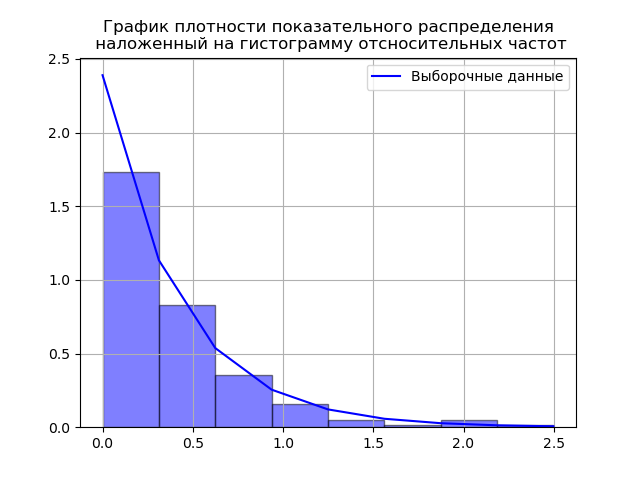
\includegraphics[width=1.0\textwidth]{../latex/inc/generated/img/relFreqDensity2.png}%
\end{figure}

%
\begin{changemargin}{-4cm}{0cm}\small{%
\begin{tabular}{|c|c|c|c|c|c|}%
\hline%
$k$&Интервал&$w_k$&$p_{k}^*$&$|w_i-p_{i}^*|$&$\frac{N(w_k - p_k)^2}{p_{k}^*}$\\%
\hline%
1.00000&{[}0.00000, 0.31228{]}&0.54000&0.52587&0.01413&0.07596\\%
\hline%
2.00000&{[}0.31228, 0.62457{]}&0.26000&0.24933&0.01067&0.09131\\%
\hline%
3.00000&{[}0.62457, 0.93685{]}&0.11000&0.11822&0.00822&0.11420\\%
\hline%
4.00000&{[}0.93685, 1.24914{]}&0.05000&0.05605&0.00605&0.13061\\%
\hline%
5.00000&{[}1.24914, 1.56142{]}&0.01500&0.02658&0.01158&1.00833\\%
\hline%
6.00000&{[}1.56142, 1.87370{]}&0.00500&0.01260&0.00760&0.91685\\%
\hline%
7.00000&{[}1.87370, 2.18599{]}&0.01500&0.00597&0.00903&2.72731\\%
\hline%
8.00000&{[}2.18599, 2.49827{]}&0.00500&0.00539&0.00039&0.00554\\%
\hline%
{-}&{-}&$\sum w_k=$1.00000&$\sum p_{k}^*=$1.00000&$max | w_i - p_{i}^*|=$0.01413&$\frac{N(w_k - p_k)^2}{p_{k}^*}$=5.07011\\%
\hline%
\end{tabular}%
\newline%
\newline%
%
}\end{changemargin}%
$m=8 \quad l=m-2=6$

%
$\chi_{B}^2 = 5.07011 \quad \chi^2_{\text{кр}, \alpha}(6) = 12.60000$

%
$5.07011 \le 12.6$%
, то гипотеза о соответствии выборки показательному распределению не противоречит экспериментальным данным при уровне значимости $a=0,05$